\documentclass[prl,aps,twocolumn,floatfix,amsmath,amssymb,superscriptaddress,tightenlines]{revtex4}
\usepackage{graphicx}
\usepackage{epstopdf}
\usepackage{amsfonts}
\usepackage{bm}
\usepackage{color}
\usepackage{ulem}
\begin{document}

\date{\today}
\title{Logarithmic terms in the entanglement entropy in
  two-dimensional gapless systems}

\author{Hyejin Ju}
\affiliation{University of California, Santa Barbara, CA, 93106}

\author{Ann B. Kallin}
\affiliation{Department of Physics and Astronomy, University of Waterloo, Ontario, N2L 3G1, Canada} 

\author{Paul Fendley}
\affiliation{Physics Department, University of Virginia,
  Charlottesville, VA 22904}
\affiliation{Microsoft Research, Station Q, CNSI Building, University of California, Santa Barbara, CA, 93106}

\author{Matthew B. Hastings}
\affiliation{Microsoft Research, Station Q, CNSI Building, University of California, Santa Barbara, CA, 93106}

\author{Roger G. Melko}
\affiliation{Department of Physics and Astronomy, University of Waterloo, Ontario, N2L 3G1, Canada} 

\begin{abstract} 
We show that the entanglement entropy of a variety of two-dimensional
gapless systems contains a logarithmic term that is not a ``boundary''
effect. Precisely, we show that the Renyi entropy between two regions
of length $l$ and $L-l$ extending around a cylinder of length $L$ depends on
$\ln(\sin(\pi l/L))$. This logarithmic term is thus akin to that
appearing in 1d systems with conformal symmetry. We illustrate this
with numerical results on the Heisenberg model with N\'eel order, a
free Dirac fermion, and the nearest-neighbor RVB wave function.


 
\end{abstract}
\maketitle


\begin{figure}[h]
  \begin{center}
  \scalebox{1}{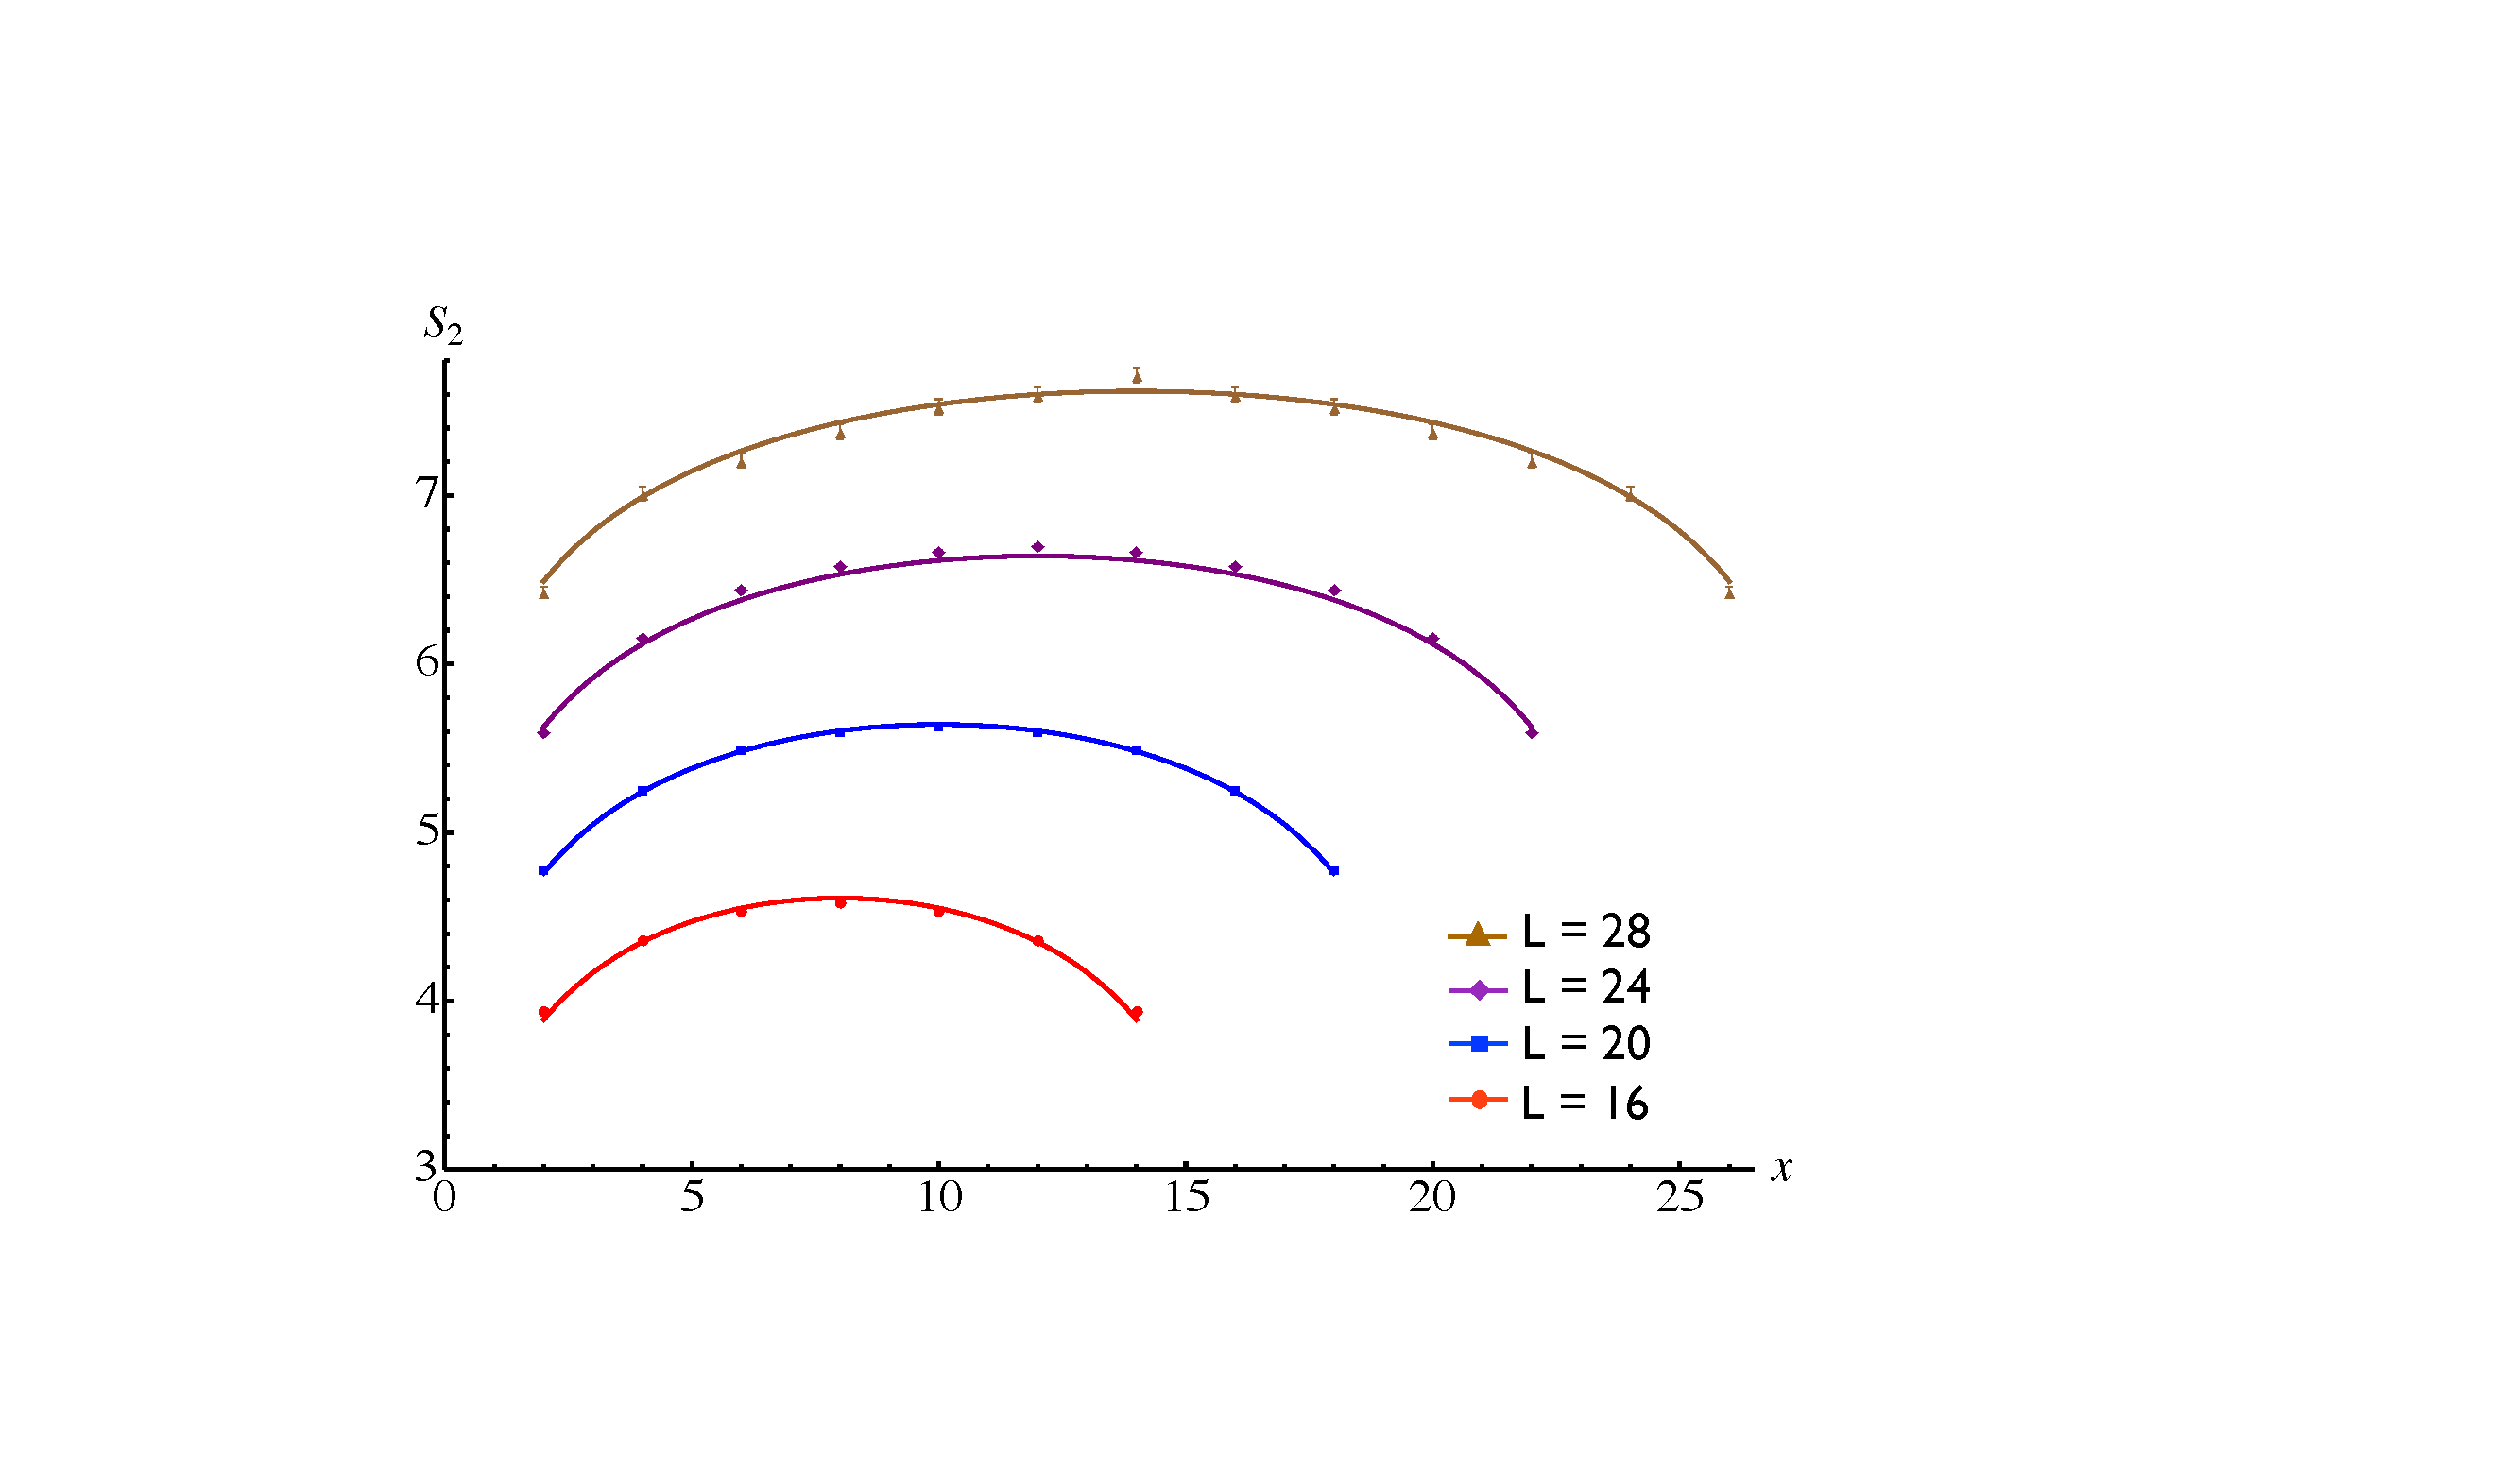
\includegraphics[width=\columnwidth]{./figs/RVB-renyibow.pdf}}
  \end{center}
  \caption{RVB Renyi-bow. Fit to $a L + b + c \ln \left( L \sin \left( \frac{\pi
 x}{L} \right) \right).$ Coefficients: $a = 0.216\pm 0.002, \, b = -9.22 \pm 0.0
4, \, c = 0.75\pm 0.02$.}
  \label{fig:1}
\end{figure}

\begin{figure}[h]
  \begin{center}
  \scalebox{1}{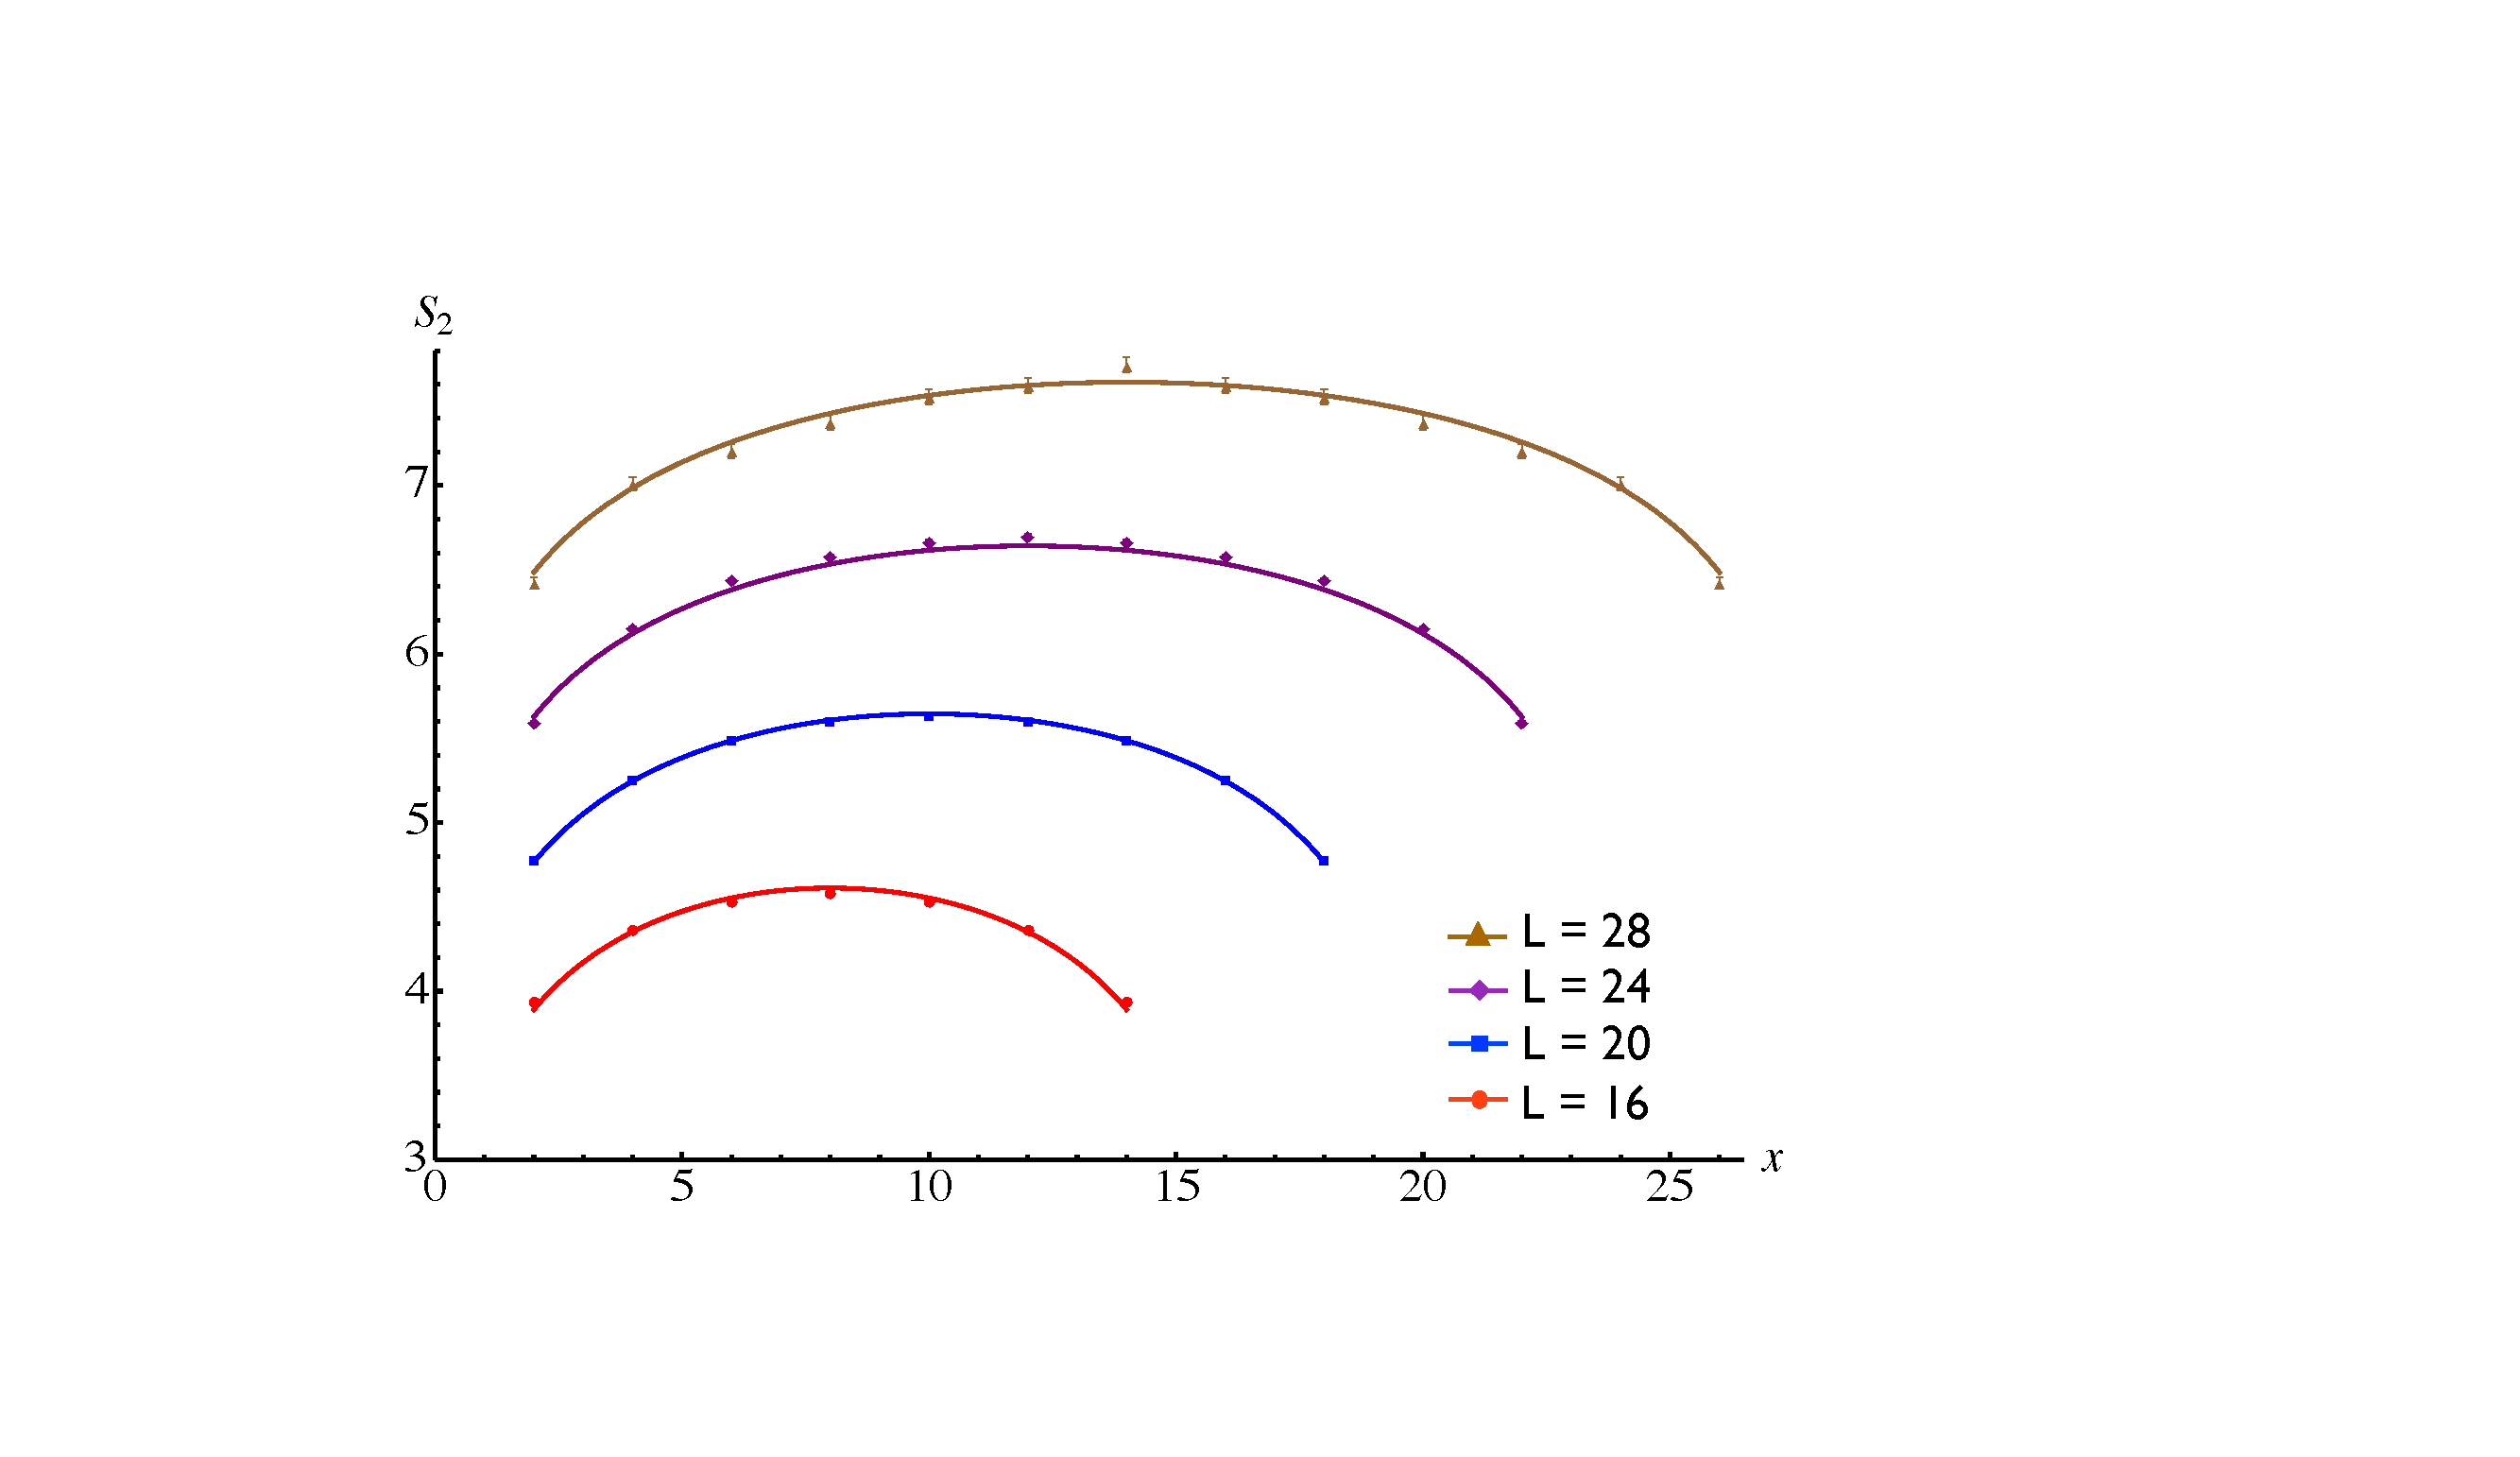
\includegraphics[width=\columnwidth]{./figs/RVB-renyibow-2.pdf}}
  \end{center}
  \caption{RVB Renyi-bow: 2. Fit to $a L + b + c \ln L + d \ln \left( \sin \left
( \frac{\pi x}{L} \right) \right).$ Coefficients: $a = 0.21\pm 0.01, \, b = -1.2
 \pm 0.4, \, c = 0.9\pm 0.2, \, d = 0.75 \pm 0.02$.}
  \label{fig:2}
\end{figure}

\begin{figure}[h]
  \begin{center}
  \scalebox{1}{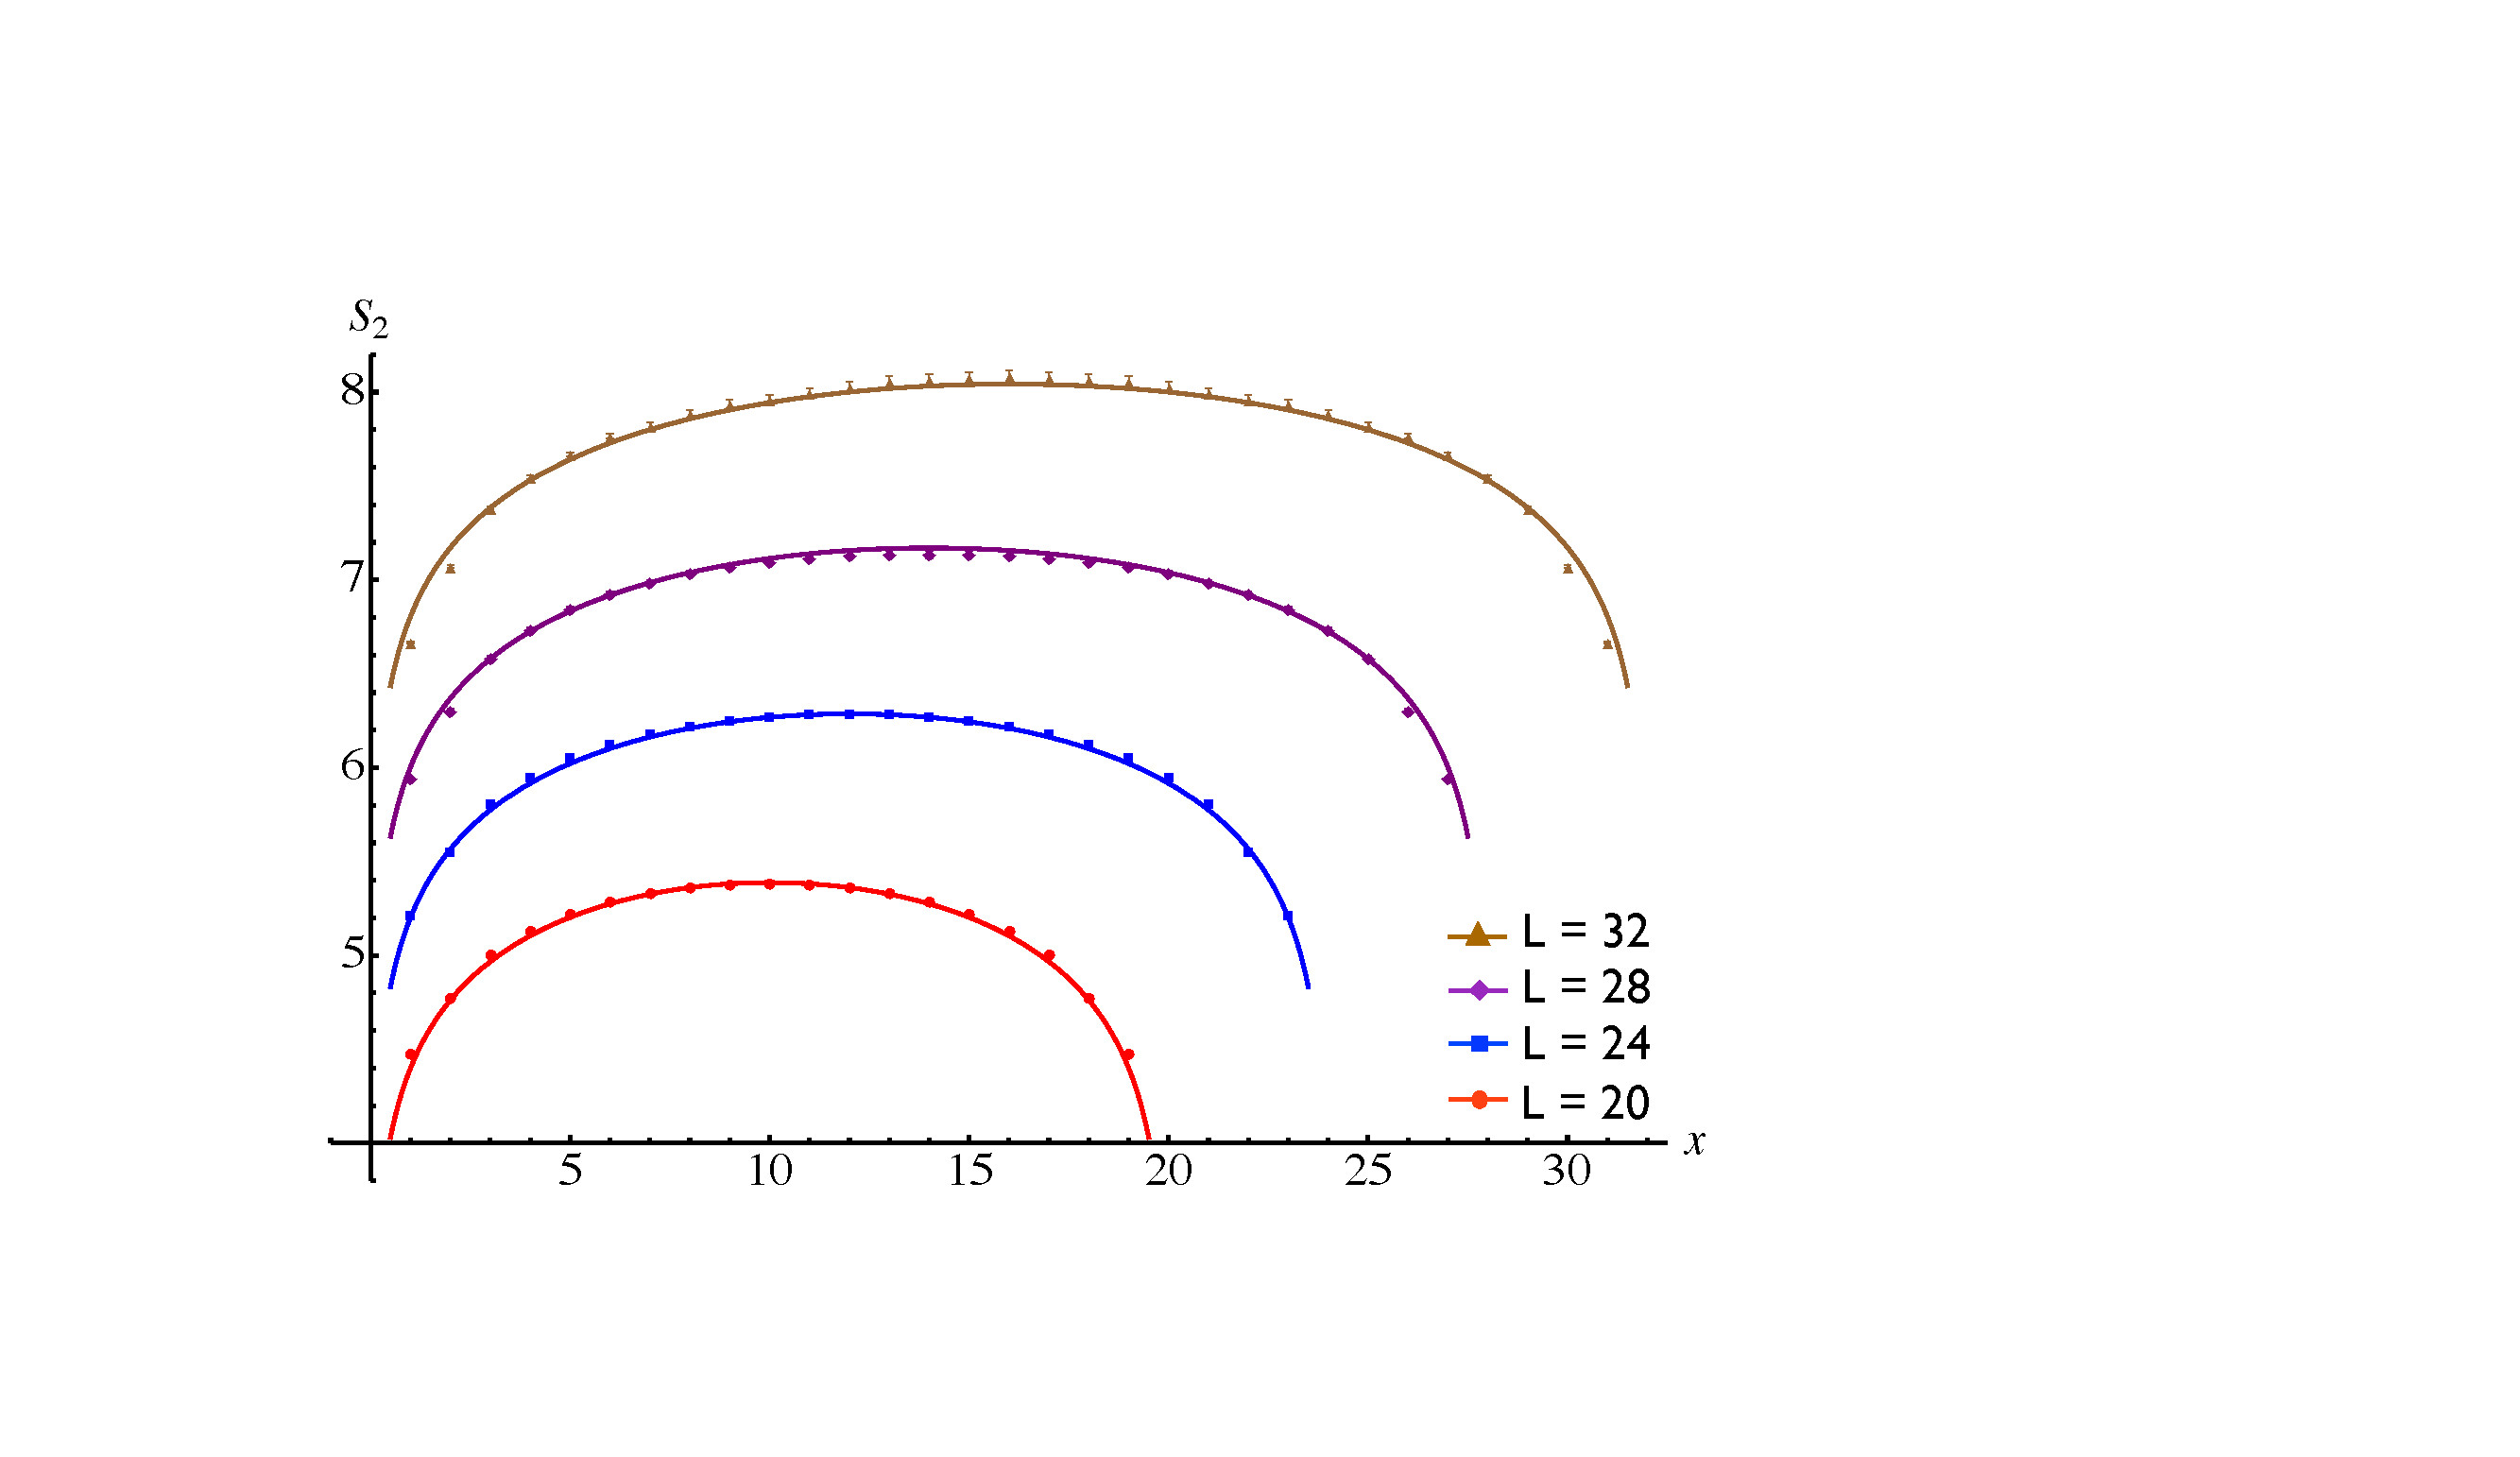
\includegraphics[width=\columnwidth]{./figs/Heisenberg-renyibow.p
df}}
  \end{center}
  \caption{Heisenberg Renyi-bow. Fit to $a L + b + c \ln \left( L \sin \left( \f
rac{\pi x}{L} \right) \right).$ Coefficients: $a = 0.2004\pm 0.004, \, b = -0.22
 \pm 0.01, \, c = 0.533\pm 0.004$.}
  \label{fig:3}
\end{figure}

\begin{figure}[h]
  \begin{center}
  \scalebox{1}{\includegraphics[width=\columnwidth]{./figs/Heisenberg-renyibow-2
.pdf}}
  \end{center}
  \caption{Heisenberg Renyi-bow-2. Fit to $a L + b + c \ln L + d \ln \left( \sin
 \left( \frac{\pi x}{L} \right) \right).$ Coefficients: $a = 0.197\pm 0.003, \, 
b = -0.4 \pm 0.1, \, c = 0.61\pm 0.06, \, d = 0.533 \pm 0.004$.}
  \label{fig:4}
\end{figure}






\bibliography{Biblio}

\end{document}
